\section{Lösungsansatz}
\label{sec-4}
Nachdem in den vorangegangenen Kapiteln die Hintergründe erläutert und Probleme identifiziert wurden, beschreibt dieses Kapitel nun den gewählten Lösungsansatz. Der Abschnitt ist dazu wie folgt strukturiert:
Zunächst verfeinert der folgende Abschnitt den prinzipiellen Lösungsansatz und beschreibt, wie die AR-Aspekte genutzt werden sollen. Danach werden die getroffenen Designentscheidungen bezüglich dessen vorgestellt, was angezeigt wird, wie es dargestellt wird und wie damit interagiert wird.

\subsection{Design der AR-Umgebung}
\label{sec-4-1}
Ziel ist es, die AR-Technologie der HoloLens zu nutzen, um physikalische Eigenschaften darzustellen, in ihren realen Kontext einzubetten und dadurch einen räumlichen und zeitlichen Zusammenhang zu schaffen. Um dies zu realisieren werden zusätzliche, virtuelle Objekte mit der HoloLens in die Versuchsaufbauten integriert und dazu in Beziehung gesetzt. Das Zusammenspiel von realen und virtuellen Objekten bestimmt dann die Nutzererfahrung.\\

Um den räumlichen Zusammenhang herzustellen, sind die virtuellen Objekte in Relation zum Versuchsaufbau, vor allem zur Spule, zu platzieren. Dementsprechend muss die Position und Ausrichtung relevanter Geräte bestimmt und in das Koordinatensystem der Anwendung transformiert werden. Nachdem dies einmal erfolgt ist, muss der Vorgang im Laufe der Anwendung nicht wiederholt werden, denn der Aufbau wird im Laufe des Versuches nicht bewegt oder gedreht und die HoloLens verankert die Objekte an ihrer Position im Raum. Der Anwender kann sich dann frei um die Gerätschaften herum bewegen, sie aus verschiedenen Perspektiven betrachten und damit interagieren. Die Interaktion erfolgt dabei sowohl mit den realen als auch den virtuellen Objekten.\\

Neben dem räumlichen Zusammenhang wird auch ein zeitlicher hergestellt. Dies geschieht, indem die Brille in Echtzeit Messwerte von den Geräten des Versuches erhält. Diese werden dann verarbeitet und dazu in Zusammenhang stehende Darstellungen angepasst. Im Laufe des Experimentes ändert die durchführende Person die anliegende Spannung durch einen Regler an der Spannungsquelle. Das bedeutet, dass der Nutzer beim Einstellen des Stromflusses die Änderungen an den physikalischen Eigenschaften gleichsam in der Realität als auch der virtuellen Realität in Echtzeit beobachten kann.\\

Dieses Konzept macht von den zentralen Stärken der HoloLens Gebrauch. Als Head Mounted Display mit transparenter, stereoskopischer Anzeige und dem Raumverständnis sind solch immersive Anwendungsszenarien die Kernkompetenz der Brille. 

\vspace{8px}
\begin{center}
	\fbox{
		\parbox{0.9\linewidth}{
		\vspace{4px}
		\textbf{Zusammenfassung}
		\begin{itemize}[rightmargin=12px, topsep=-12px]
			\setlength{\itemsep}{-1pt}
			\singlespacing
			\item Integration von realen und virtuellen Objekten in eine Augmented Reality Anwendung
			\item Virtuelle Objekte werden in den Versuchsaufbau eingebettet und interagieren mit diesem in Echtzeit
			\item Gemessene, berechnete und beobachtete physikalische Vorgänge werden somit in einer Anwendung integriert
			\item Nutzer kann sich mit der HoloLens frei im Raum bewegen und mit der Anwendung sowie den Gerätschaften interagieren
		\end{itemize}
	\vspace{18px}
	}}\\
\end{center}
\vspace{6px}


Unter diesem grundsätzlichen Ansatz soll die Lösung nun weiter konkretisiert werden.


\subsection{Inhaltliches Design} %Dargestellte Informationen
Zunächst ist zu entscheiden, welche physikalischen Eigenschaften durch die HoloLens visualisiert werden sollen. Von besonderem Interesse sind hier vor allem Informationen, die für den Versuch zwar relevant, für den Nutzer jedoch nicht direkt beobachtbar sind.\\

Das betrifft in erster Linie die beiden sich überlagernden Magnetfelder von Erde und Spule. Das Zusammenspiel beider Felder und deren Eigenschaften ist elementar für das Verständnis des Experimentes. Allerdings sind Magnetfelder nicht sichtbar und die Auswirkungen auf die Magnetnadel entstehen durch das überlagerte Feld, die einzelnen Komponenten des Feldes sind darin nicht mehr erkennbar. Deshalb sollen diese für den Anwender sichtbar gemacht werden. In Absprache mit Experten wurde entschieden, zunächst nur die Einzelfelder und nicht das resultierende Feld zu visualisieren \autocite{Reinholz18}.\\
\noindent\hspace*{5mm}
Damit die Felder auch als solche interpretiert und ihre Eigenschaften erkannt werden können, wird auf die etablierten Darstellungsmodelle über Feldlinien bzw. Vektoren zurückgegriffen. Da die Modelle sowohl Vor- als auch Nachteile haben, sollen beide Darstellungen alternativ angeboten werden.\\

Die Auslenkung des Kompass hängt von Richtung und Stärke der beiden Einzelfelder in unmittelbarer Nähe des Kompasses ab. Diese Eigenschaften der Felder sind damit für den Versuch ausschlaggebend und sollen deshalb dargestellt werden.\\
\noindent\hspace*{5mm}
Während die Stärke und Richtung des Erdmagnetfeldes an einem Ort als konstant angenommen werden kann, ändert sich das Feld der Spule mit der Stromstärke. Stärke und Richtung des Feldes hängen direkt von der anliegenden Stromstärke und der Richtung des Stromflusses ab. Um diesen Zusammenhang sichtbar zu machen, soll die dargestellte Feldstärke (des Feldes der Spule) anhand von gemessenen Echtzeitdaten angepasst werden. Dafür soll die aktuell gemessene Stromstärke an die HoloLens übermittelt werden. Aus dieser lässt sich anhand der Gleichung \ref{eq:mfield} in Abschnitt \ref{sec-2-3-3} die Feldstärke für den Mittelpunkt der Spule berechnen.\\

Für die Auslenkung der Nadel ist lediglich das Feld in unmittelbarer Nähe des Kompass ausschlaggebend. Deshalb beschränken sich die Repräsentationen der Felder zunächst auf das Innere der Spule. In diesem ist das Feld nahezu homogen, was ebenfalls erkennbar sein soll. Vor diesem Hintergrund und dem Ziel eines qualitativen Verständnisses kann die Feldstärke im Mittelpunkt für einen größeren Bereich im Inneren der Spule angenommen werden.\\

Um unabhängig von der Durchführung des Experimentes auch einen Eindruck von der Struktur des gesamten, durch die Spule erzeugten Feldes zu vermitteln, wird eine Darstellung von Simulationsdaten verwendet. Diese legt eine numerisch berechnete Lösung zu Grunde, die dieser  Arbeit zur Verfügung steht. Ziel der Darstellung ist es, die Homogenität im Inneren der Spule im Gegensatz zur Inhomogenität des restlichen Feldes sichtbar zu machen. Hier folgt das Design der Empfehlung von Experten, diese Eigenschaft ebenfalls sichtbar zu machen \autocite{Reinholz18}. Denn auch wenn das Feld außerhalb der Spule keinen Einfluss auf die eigentliche Durchführung des Experimentes hat, so unterstützt es dennoch das Verständnis, warum der Kompass gerade in der Mitte der Spule aufgestellt wird.\\

Ein weiterer interessanter Aspekt ist die Einbindung theoretischer Ergebnisse. Das ermöglicht dem Anwender, direkt am Versuchsaufbau sowohl gemessene, als auch berechnete Werte zu erfassen und beide miteinander zu vergleichen. Bei der Bestimmung des Erdmagnetfeldes betrifft das vor allem die Auslenkung des Kompasses, die sich in Abhängigkeit des Feldstärkevektors verändert. Die Magnetnadel des Kompass unterliegt dabei Faktoren wie Reibung und Trägheit, die zu Abweichungen führen können. Ein berechneter, virtueller Kompass unterliegt solchen Einschränkungen nicht und kann ergänzend zum realen Konterpart das angenommene Verhalten des Systems unter Idealbedingungen aufzeigen. Deshalb soll ein solcher durch die HoloLens integriert werden.\\

Zusammenfassend sollen also die folgenden Elemente visualisiert werden:
\begin{enumerate}
	\item Die einzelnen Magnetfelder von Erde und Spule werden in einem Bereich im Inneren der Spule dargestellt. Die Darstellungen erfolgen sowohl über das Feldlinien- als auch das Vektormodell und ändern sich dynamisch mit der eingestellten Spannung. Dabei sollen die folgenden Eigenschaften der Felder erkennbar sein:
	\begin{itemize}[topsep=-0.25em]
		\setlength{\itemsep}{-0.25em}
		\item Stärke
		\item Richtung
		\item Homogenität
	\end{itemize}
	\item Das Feld der Spule soll außerdem gesondert auf Basis von Simulationsdaten für einen größeren Bereich auch außerhalb der Spule dargestellt werden. Dafür wird das Feldlinienmodell und eine bestehende Simulation genutzt.
	\item Die Richtung des Stromflusses durch die Spule wird durch einen Indikator. Ergänzend dazu sollen Plus und Minus gekennzeichnet werden.
	\item Die berechnete Auslenkung einer theoretischen, idealen Magnetnadel ohne Störeinflüsse. 
	\item Die gemessenen und berechneten Werte für Stromstärke und Flussdichte.
\end{enumerate}
\vspace{6px}

%Diese Entscheidungen wurden in Zusammenarbeit mit Experten validiert.
Für diese Elemente gilt es nun ein visuelles Design zu konzipieren und eine technische Realisierung zu erarbeiten. Diese werden jedoch durch Designentscheidungen beeinflusst, die technische Eigenschaften der HoloLens adressieren, um eine komfortable Nutzung zu gewährleisten. Deshalb soll zunächst auf diese näher eingegangen werden.

\subsection{Designentscheidungen im Hinblick auf die HoloLens}
\label{sec-4-2}
Viele Darstellungen sollen am Versuchsaufbau, also vor allem an der Spule, verankert werden. Das bedeutet, dass der Anwender Abstand und Blickwinkel zu diesen Objekten durch seine Bewegungen und Blickrichtung selbst steuert. Um dennoch stets eine komfortable Nutzung zu ermöglichen, und die zuvor erläuterten Probleme im Hinblick auf Distanz und Blickrichtung zu vermeiden, werden mehrere Maßnahmen getroffen.\\

\textit{Distanz}\\
Um zu geringe Distanzen zwischen Nutzer und den virtuellen Objekten zu vermeiden, werden fest verankerte Darstellung unterhalb einer gewissen Distanz ausgeblendet. Hier folgt das Design den existierenden, zuvor aufgeführten Empfehlungen. Das ermöglicht dem Nutzer zugleich das Eintauchen in die Darstellungen. Frei bewegliche Elemente hingegen werden durch entsprechende Skripte den Bewegungen des Nutzers angepasst, so dass sie stets in einer komfortablen Zone des Sichtfeldes verbleiben.\\

Weiterhin soll eine Nutzung im Abstand von ca. 1,2m bis 1,5m begünstigt werden. Das hat mehrere Gründe. Zum einen passt bei diesem Abstand die Spule vollständig in das Sichtfeld der HoloLens. Darin eingebettete Darstellungen werden also nicht durch die Grenzen des Field of View abgeschnitten. Dabei bleibt auch noch etwas Spielraum für Kopfbewegungen, so dass die Darstellungen nicht schon bei kleinen Bewegungen an die Grenzen des Displays stoßen. Gleichzeitig bleiben nicht so große Teile des Sichtfeldes ungenutzt. Außerdem reduzieren sich so die Effekte durch die Diskrepanz zwischen Konvergenz und Akkommodation der Augen im Vergleich zu kleineren Abständen. Hier findet also ein Kompromiss zwischen Ausnutzung des Sichtfeldes und Komfort statt. Der genannte Bereich wurde dabei aus praktischer Erfahrung festgelegt.\\

\textit{Größe \& Blickrichtung}\\
Für die Darstellungen bedeutet das, dass die Größe der Objekte für diesen Bereich geeignet sein sollte. Darüber hinaus kann die Auswahl eines geeigneten Tisches die Nutzung begünstigen. Das Design geht davon aus, dass der Nutzer die Anwendung im Stehen verwendet, damit er in der Lage ist, sich frei um den Versuchsaufbau herum zu bewegen. Ein entsprechend hoher Tisch führt dazu, dass der vertikale Blickwinkel im empfohlenen Bereich zwischen 0° und 35° unterhalb der Horizontlinie liegt. Weiterhin kann die Spule mit etwas Abstand zur Tischkante positioniert werden, um so auf natürliche Weise die Nutzung in der geeigneten Distanz zu begünstigen.\\

\textit{Farbe}\\
Die Farbe bestimmt auf der HoloLens nicht nur die Helligkeit, sondern auch die Transparenz eines Objektes. Bei der Farbwahl wird deshalb darauf geachtet, dass Objekte, die gleich transparent erscheinen sollen, auch gleich hell sind. Das geschieht, indem die Farben so gewählt werden, dass sich die drei RGB-Farbkomponenten zu einem konstanten Wert addieren.\\

Nach diesen allgemeinen Designentscheidungen, die alle Visualisierungen betreffen, kann nun das visuelle Design konkretisiert werden.

\subsection{Visuelles Design}
Für die im vorangegangenen Abschnitt \ref{sec-4-2} erarbeiteten Elemente sollen nun konkrete Darstellungen konzipiert werden.\\

\subsubsection{Feldliniendarstellung}
\label{sec-4-4-1}
Im Inneren der Spule sollen die Komponenten des Magnetfeldes über dynamische Feldlinien dargestellt werden. Dies geschieht, indem 3D-Objekte räumlich in der Spule positioniert werden. Diese Einbettung wird unterstützt, indem eine Verdeckungsberechnung erfolgt, so dass räumlich hinter Teilen der Spule positionierte durch diese überdeckt werden. Außerdem werden die Objekte schattiert, damit die Form und Ausrichtung im Raum erkennbar wird. Dieses Vorgehen dient dazu, die gewünschte räumliche Einbettung zu erzielen.\\

\textit{Form, Größe und Farbe}\\
Die Form orientiert sich an dem etablierten Darstellungsmodell und besteht daher aus einem länglichen Zylinder mit integrierten Pfeilköpfen. Die Größe der Objekte wurde anhand von Erfahrungswerten angepasst. Durchmesser und Länge sind vergleichbar mit denen eines Kugelschreibers oder dickeren Stiftes. Um die Felder von Erde und Spule unterscheiden zu können, wurden mit Hellblau und Orange unterschiedliche Farben für die Objekte gewählt. Blau wird oft für Magnetfeldlinien verwendet und daher auch hier gebraucht. Allerdings wird ein weniger gesättigtes, helleres Blau verwendet, damit die Deckkraft vor helleren Hintergründen nicht verloren geht. Das Orange weißt die selbe Helligkeit wie das Blau auf, damit sich die Objekte nicht in der Transparenz voneinander unterscheiden.\\
\noindent\hspace*{5mm}
Die folgenden Erörterungen beziehen sich zunächst auf der Feld der Spule.\\

\textit{Anordnung}\\
Die Feldlinien der Spule verlaufen orthogonal zur X-Y-Ebene, also in Richtung der Z-Achse. Damit die gewünschten Eigenschaften (Stärke, Homogenität und Richtung) des dreidimensionalen Feldes anhand des Feldlinienmodells erkennbar sind, bedarf es mindestens vier Linien. In einer 2x2 Anordnung um den Mittelpunkt der X-Y-Ebene ist so der Abstand in beiden Dimensionen sichtbar und die Linien sind symmetrisch zur Z-Achse. Anhand der Parallelität lässt sich die Homogenität erkennen und anhand des Abstandes (in der horizontalen oder vertikalen, beide sind gleich groß) die Stärke. Die Flussrichtung ist über die eingebauten Pfeilspitzen abgebildet. Als Darstellungsvolumen wurde ein zylindrischer Ausschnitt der Spule gewählt, da diese den Raum besser ausfüllt, als beispielsweise ein kubischer Ausschnitt.\\

\textit{Anzahl}\\
Bei einem festen, für die Darstellungen zur Verfügung stehenden Volumen und kleiner werdenden Abständen müssen zunehmend mehr Linien gezeichnet werden. Zu viele Objekte würden jedoch die Sichtbarkeit anderer Elemente wie Magnetnadel und Kompass beeinträchtigen. Außerdem transportieren zusätzliche Feldlinien keine zusätzlichen Informationen (im Fall eines homogenen Feldes). Allerdings unterstützt die Beobachtung, dass mit zunehmender Flussdichte die Anzahl der Feldlinien steigt, das Verständnis des Feldlinienmodells. Daher wurde für die Umsetzung das Intervall von minimalem und maximalem Abstand so gewählt, dass mindestens 4 und höchstens 16 Linien dargestellt werden. Beim Ein- und Austreten der Objekte in das bzw. aus dem Darstellungsvolumen werden sie kontinuierlich ein bzw. ausgeblendet.\\

\textit{Feld der Erde}\\
Um das Feld der Erde darstellen zu können, wird ein fester Wert für dessen Flussdichte angenommen. Da das Feld statisch ist, wird es über die minimal notwendige Anzahl an Feldlinien repräsentiert. Zusätzliche Linien würden aufgrund der Homogenität keine weiteren Informationen transportieren. Einen Eindruck der Feldlinien und deren Transparenz beim Ein- bzw. Austritt in den Darstellungsbereich vermittelt Abbildung \ref{img:mfield-lines}.

\begin{figure}[h!]
	\centering
	\includegraphics[width=0.8\textwidth]{images/unity/fieldlines.jpg}
	\caption{Feldlinien}
	\label{img:mfield-lines}
\end{figure}

\textit{Skalierung}\\
Bei der Repräsentation der Flussdichte wurde sich bewusst für die Abbildung auf den Abstand der Feldlinien entschieden. Oft wird statt des Abstandes die Anzahl der durch eine Einheitsfläche verlaufenden Feldlinien proportional zur Flussdichte gewählt. Da für den Anwender in erster Linie jedoch der Abstand die sichtbare, sich ändernde Größe ist, würde dies den falschen Eindruck erwecken, die Flussdichte ändere sich nicht linear mit der Stromstärke. Daher wurde sich für die proportionale Änderung des Abstandes entschieden.\\

\textit{Begrenzung der Darstellung}\\
Die Visualisierung des Feldes erfordert die Festlegung eines darzustellenden Bereiches für die Flussdichte. Voreingestellt ist ein Bereich von $5 \mu T$ bis $60 \mu T$, die Flussdichte der Erde liegt mit $30 \mu T$ bis $40 \mu T$ im mittleren Bereich dieser Skala. Am unteren Ende des Bereiches werden die Objekte über Transparenz ausgeblendet. Auf diese Weise soll angedeutet werden, dass nur die Darstellungen verschwinden, nicht jedoch die physikalischen Sachverhalte, die repräsentiert werden.\\
\noindent\hspace*{5mm}
Nach oben hin ist keine Darstellung der Begrenzung vorgesehen. Der Bereich sollte so gewählt werden, dass die obere Grenze durch die maximal am Regler einstellbare Stromstärke nicht erreicht werden kann. Somit erfährt der Anwender die Limitierung der Darstellung auf natürliche Weise. Die Konfiguration der Schaltung kann hier über eingebaute Widerstände so an die Spannungsquelle angepasst werden, dass der erzeugte Stromfluss im gewünschten Bereich liegt. Diese Begrenzung gilt nicht nur für die Feldlinien, sondern alle an die Flussdichte bzw. Stromstärke gekoppelten Elemente, sodass ein konsistentes Verhalten entsteht.

\vspace{4px}
\begin{center}
	\fbox{
		\parbox{0.9\linewidth}{
			\vspace{4px}
			\textit{Zusammenfassung}
			\begin{itemize}[rightmargin=12px, topsep=-12px]
				\setlength{\itemsep}{-1pt}
				\singlespacing
				\item 3D-Pfeillinien repräsentieren Feldlinien über Abstand und Ausrichtung
				\item Räumlich Einbettung in die Spule durch Positionierung und Verdeckung
				\item Unterscheidung der Komponenten über verschiedene Farben
				\item Änderung des Abstandes proportional zur Feldstärke über Kontraktion zur Z-Achse
				\item Linien werden über Transparenz an den Darstellungsgrenzen ein- bzw. ausgeblendet
			\end{itemize}
			\vspace{18px}
	}}\\
\end{center}
%\vspace{6px}

\subsubsection{Vektordarstellung}
\label{sec-4-4-2}
Neben der dynamischen Feldliniendarstellung soll das Feld auch über Vektoren repräsentiert werden. Die Realisierung erfolgt dabei ebenfalls über 3D-Objekte, die sich nur in der Form von denen der Feldlinien unterscheiden. Damit die Vektoren als solche erkennbar sind, wurde eine Repräsentation als 3D-Pfeil gewählt.
 
\textit{Anordnung, Anzahl und Skalierung}\\
In der Vektordarstellung werden mindestens acht Vektoren benötigt, jeweils zwei pro Raumrichtung, damit die gewünschten Eigenschaften des Feldes erkennbar werden. Die Anordnung erfolgt in einem 3D-Gitter, bei dem die Anzahl und die Abstände pro Dimension parametrisiert sind. Auch hier gilt, dass mehr Objekte im homogenen Teil des Feldes keine weiteren Informationen transportieren. Deshalb wurde die minimal notwendige Anzahl von acht Vektoren gewählt.\\
\noindent\hspace*{5mm}
Die Flussdichte wird im Fall der Pfeile über deren Länge ausgedrückt. Die Form der Objekte soll mit einer sich ändernden Länge nicht verzerrt werden. Eine einfache Skalierung der Pfeillänge würde jedoch dazu führen, dass auch die Pfeilspitze in die Länge gezogen wird. Daher wird die Geometrie zur Laufzeit angepasst und nur ein Teil in der Mitte verändert. Das Design ist in Abbildung \ref{img:mfield-vectors} abgebildet.\\

\begin{figure}[h!]
	\centering
	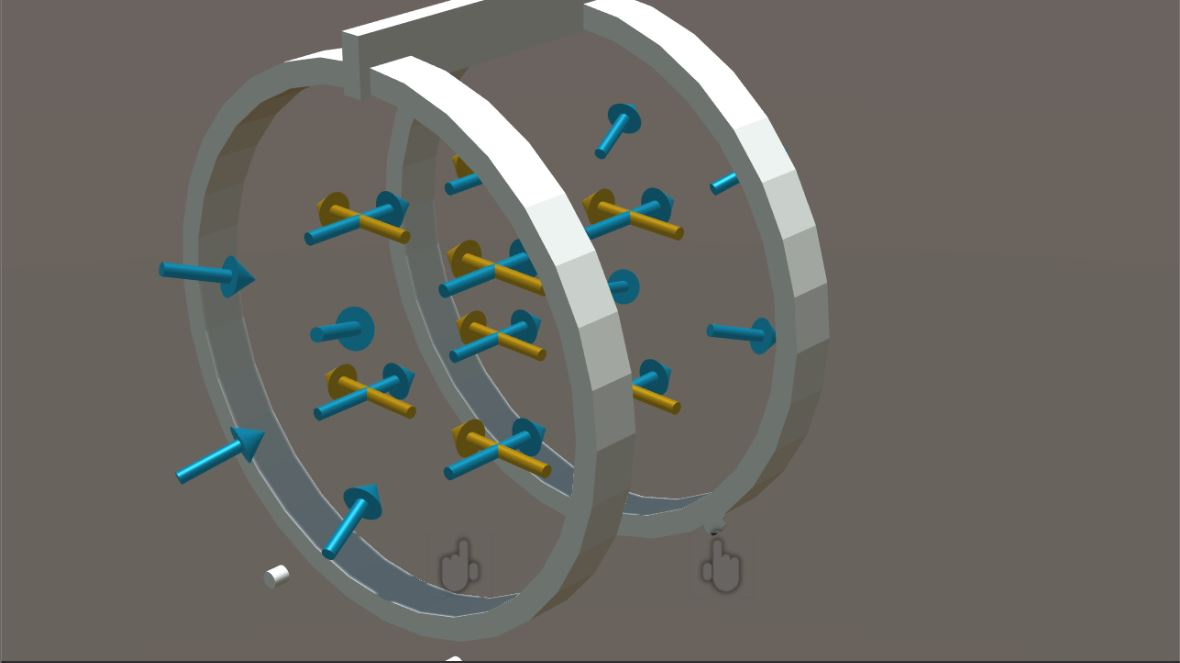
\includegraphics[width=0.8\textwidth]{images/unity/vector.jpg}
	\caption{Feldlinien}
	\label{img:mfield-vectors}
\end{figure}

\textit{Bezugspunkt}\\
Welcher Punkt dem Vektor als Ankerpunkt dient ist dabei nicht entscheidend, denn ein Pfeil repräsentiert jeden Punkt des homogenen Feldes. Eine explizite Darstellung ist daher nicht vorgesehen. Allerdings wird die Verankerung im Mittelpunkt dadurch deutlich, dass die Position des Pfeils bei variierender Länge gleich bleibt.\\

\textit{Inhomogener Anteil}\\
Im Gegensatz zu den Feldlinien ist eine Darstellung des inhomogenen Feldes über Vektoren auch ohne aufwendige Echtzeit-Berechnungen möglich (siehe Kap. \ref{sec-2-3-2}). Die Anwendung nutzt diese Eigenschaft, um in dieser Darstellung auch das inhomogene Feld anzudeuten. Dies geschieht, indem das Raster so gewählt wird, dass vor und hinter der Spule (im Sinne der Z-Achse) jeweils eine Reihe Vektoren positioniert ist. Diese sind hier im Vergleich deutlich kürzer und nicht parallel, sondern nach innen bzw. nach außen gerichtet. So wird erkennbar, dass das Feld hier schwächer und inhomogen ist. Da die Darstellungen erst ab einem minimalen Wert eingeblendet werden, wird der inhomogene Teil nach dem homogenen Teil eingeblendet.\\
\noindent\hspace*{5mm}
Ziel dieser Maßnahme ist es, den Unterschied zwischen dem homogenen Feld im Inneren und dem inhomogenen Feld im Äußeren der Spule deutlich zu machen. Die dargestellte Richtung und Stärke der äußeren Vektoren entspricht deshalb nicht genau den tatsächlichen physikalischen Werten. Stattdessen wurden Werte gewählt, die den Unterschied besser erkennen lassen.

\vspace{4px}
\begin{center}
	\fbox{
		\parbox{0.9\linewidth}{
			\vspace{4px}
			\textit{Zusammenfassung}
			\begin{itemize}[rightmargin=12px, topsep=-12px]
				\setlength{\itemsep}{-1pt}
				\singlespacing
				\item 3D-Pfeile repräsentieren Feldstärkevektoren über Länge und Ausrichtung
				\item 8 Pfeile für homogenes Feld, weitere 8 für Andeutung inhomogenes Feld außerhalb der Spule
				\item Anordnung im 3D-Gitter mit konfigurierbaren Parametern (Abstand und Anzahl, jeweils pro Raumrichtung)
			\end{itemize}
			\vspace{18px}
	}}\\
\end{center}
\vspace{6px}

\subsubsection{Darstellung der Simulationsdaten}
\label{sec-4-4-3}
Nicht zuletzt soll das Magnetfeld der Spule über eine Darstellung vorberechneter Simulationsdaten erfolgen. Dafür steht der Arbeit eine Simulationssoftware zur Verfügung, bei der lediglich die Parameter für die Visualisierung der Feldlinien zu setzen sind.\\

\textit{Anzahl und Anordnung}\\
Die Auswahl von 12 Feldlinien erfolgte aus praktischem Ermessen bezüglich der Sichtbarkeit aus 1,5 Metern Entfernung. Dabei wurde bewusst eine gerade Anzahl gewählt. Andernfalls entsteht eine Feldlinie, die genau auf der Z-Achse liegt und nicht geschlossen ist sondern von minus nach plus Unendlich verläuft. Dies wurde aus didaktischen Gründen vermieden.\\
\noindent\hspace*{5mm}
Die Visualisierung der Simulationsdaten ist in Abbildung \ref{img:mfield-simulation} näher zu sehen, die die selben Daten mit zwei verschiedenen Farbskalen visualisiert darstellt.
\begin{figure}[h!]
	\centering
	\includegraphics[width=0.45\textwidth]{images/unity/simulation_rgb.jpg}
	\hspace{0.03\textwidth}
	\includegraphics[width=0.45\textwidth]{images/unity/simulation.jpg}
	\caption{Darstellung der Simulationsdaten. Links mittels der RGB- und rechts mittels der RG-Farbskala.}
	\label{img:mfield-simulation}
\end{figure}

\textit{Farbe}\\
Die Wahl der Farbskala fiel aus mehreren Gründen auf eine RGB-Skala. Die Linien zeigen die kontinuierliche Änderung der Flussdichte, die durch einen kontinuierlichen Farbverlauf weiter hervorgehoben werden soll. Dabei kommt es nicht auf eine unverfälschte Repräsentation oder das Ablesen der numerischen Werte an, weshalb auch keine Skala mit Farbe und den dazugehörigen Werten angezeigt wird. Es geht viel mehr um das qualitative Verständnis der Darstellung. Mit der gewählten Skala unterscheiden sich die drei wesentlichen Regionen durch ihre Farbe klar voneinander:
\begin{itemize}
	\setlength{\itemsep}{-1pt}
	\singlespacing
	\item Inhomogenes, schwaches Feld außen: Blau
	\item Homogenes, mittel-starkes Feld innen: Grün
	\item Inhomogenes, starkes Feld unmittelbar am Rand der Spule: Rot
\end{itemize}

Darüber hinaus sprechen technische Gründe für eine solche Farbskala. Damit die Linien in Helligkeit und Transparenz nicht variieren, sollten sich die Farbanteile im RGB-Raum stets zu einem konstanten Wert addieren. Die gewählte Skala erfüllt diese Eigenschaft. Gleiches gilt jedoch beispielsweise auch für die ebenfalls umgesetzte Rot-Grün-Skala.\\
\noindent\hspace*{5mm}
Entscheidend ist hier der Umstand, dass die RGB-Skala und sehr ähnliche Skalen (z.B. Regenbogen) typisch für die Feldliniendarstellung in der Physik sind (vgl. z.B. die Abb. in Kap. \ref{sec-2-2-2}) und daher in diesem fachlichen Kontext interpretierbar sind.

\subsubsection{Der Stromfluss} 
\label{sec-4-2-3}
Beim Stromfluss ist in erster Linie die Flussrichtung durch die Spulen von Interesse, denn hiervon hängt die Ausrichtung des entstehenden Magnetfeldes ab. Diese wird über an der Spule anliegende Indikatoren in Form von 2D-Pfeilen angezeigt. Abbildung \ref{img:current} verdeutlicht diesen Ansatz.\\
\noindent\hspace*{5mm}
Die Positionierung direkt auf bzw. an den Spulen führt dazu, dass kein zusätzlicher Screenspace, der für die Felddarstellung genutzt wird, in Anspruch genommen werden muss, da das Feld hier ohnehin von den Spulen verdeckt wird. Die Spulen bleiben weiterhin gut sichtbar, da nur ein Teil und nur eine Seite überdeckt wird. Hier haushaltet die Anwendung also mit dem ihr zur Verfügung stehenden Platz.\\

\begin{wrapfigure}{R}{0.5\textwidth}
	\centering
	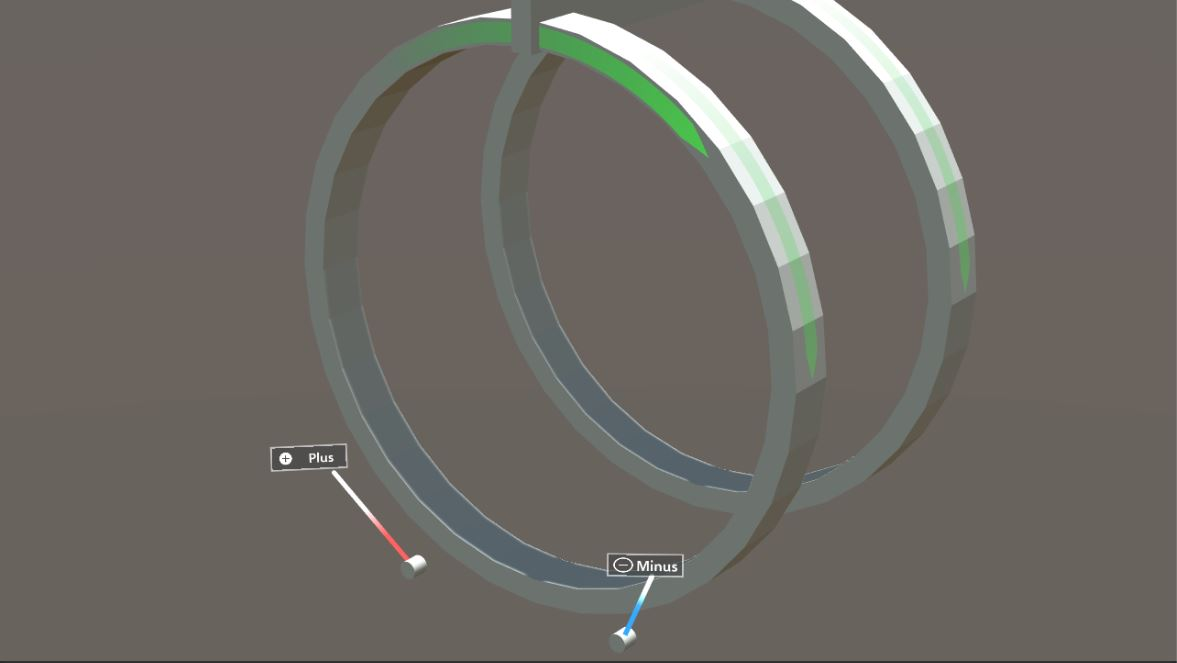
\includegraphics[width=0.45\textwidth]{images/unity/current.jpg}
	\caption{Kennzeichnung des Stromflusses an der Spule über grüne Indikator-Pfeile und Beschriftung der Anschlüsse. Aufgrund des Kamerawinkels sind die seitlich angebrachten Indikatoren fast ausgeblendet, während der frontal positionierte Indikator vollständig eingeblendet ist.}
	\label{img:current}
\end{wrapfigure}

Damit die Indikatoren aus verschiedenen Winkeln sichtbar sind, werden diese abhängig von Position und Blickwinkel des Betrachters angezeigt, wie in der Abbildung zu sehen. Bewegt sich der Nutzer um den die Spule herum, werden die Pfeile durch kontinuierlichen Übergang ein- und ausgeblendet.\\

Ein Nachteil dieser Lösung ist jedoch, dass das zuvor erläuterte Problem mit der Akkommodation auftritt. Die Kante zwischen virtuellem Pfeil und realer Spule kann bei einer Entfernung unter 2m zu Irritationen führen, da sich das Auge auf eine Akkommodation festlegen muss und dementsprechend das andere Objekt nicht als scharf wahrnimmt, obwohl beide gleich weit entfernt sind. Allerdings stehen beide Objekte selten im Fokus und die Spule muss nicht detailreich betrachtet werden, deshalb überwiegen hier die Vorteile dieser Lösung.\\

\textit{Annotationen der Anschlüsse}\\
Damit die Stromrichtung auch als technische Stromrichtung interpretiert und in die Schaltung eingeordnet werden kann, sind die Konnektoren mit Labels in Form von Tooltips mit Bezeichnung, entsprechender Farbe und Icon ausgestattet. Die Lables orientieren sich dabei zur Kamera hin, damit sie aus verschiedenen Winkeln lesbar bleiben.\\

\vspace{8px}
\begin{center}
	\fbox{
		\parbox{0.9\linewidth}{
			\vspace{4px}
			\textbf{Zusammenfassung}
			\begin{itemize}[rightmargin=12px, topsep=-12px]
				\setlength{\itemsep}{-1pt}
				\singlespacing
				\item Direkt an den Spulen verankerte Indikatoren zeigen die Stromrichtung an
				\item Indikatoren passen sich der Position des Nutzers an
				\item Kennzeichnung der Konnektoren mit Plus und Minus anhand von Labels
			\end{itemize}
			\vspace{18px}
	}}\\
\end{center}
\vspace{6px}

\subsubsection{Der Kompass} 
\label{sec-4-2-4}
Um theoretisch berechnete mit praktisch bestimmten Werten vergleichen zu können, wird ein virtueller Kompass in den Versuch integriert. Um dies zu realisieren wählt diese Lösung einen umfassenderen Ansatz: Der Kompass bildet sich aus einem Zusammenspiel der realen Magnetnadel und einer virtuellen Skala. Die Auslenkung der realen Nadel wird also anhand einer eingebetteten, virtuellen Skala abgelesen.\\

Dieses Vorgehen hat vor allem zwei Gründe. Erstens wäre eine herkömmliche, unter der Nadel angebrachte Skala nur schwer lesbar. Das liegt an der gewünschten Entfernung, aus der die Nutzung erfolgen soll, da hierfür die Skalen oft zu klein sind. Dazu kommt der flache angestrebte Blickwinkel. Letzterer ist viel geringer als die steilen Winkel, die normalerweise zum Ablesen der Richtung benötigt werden.\\
\noindent\hspace*{5mm}
Zweitens würde eine ausreichend große Skala Platz im inneren der Spule einnehmen. Dieser Platz wird jedoch für die Felddarstellungen benötigt. Eine virtuelle Skala hingegen lässt sich entsprechend dieser Bedürfnisse konzipieren. Außerdem lässt sich darin direkt eine weitere, theoretisch berechnete Auslenkung markieren. Gleichzeitig bleibt die reale Nadel nutzbar. Diese ist mit $12 cm$ Länge bewusst groß genug gewählt, damit sie gut zu sehen ist. Außerdem wurde die zuvor schwarze Nadel weiß überklebt, damit sie zwischen den Hologrammen besser zu sehen ist.\\

Die virtuelle Skala wurde als Ring unmittelbar um die Spule herum designet, um keinen zusätzlichen Platz im Inneren der Spule zu beanspruchen und gleichzeitig möglichst wenig zusätzliches Sichtfeld in Anspruch zu nehmen. Denn je größer ein Objekt, desto eher wird es an den Grenzen des Sichtfeldes abgeschnitten.\\
\noindent\hspace*{5mm}
Um die wichtigen Auslenkungen erkennbar zu machen, werden dafür Hilfslinien gezeichnet. Das betrifft Auslenkungen von 0 und 45 Grad. Denn Ziel des Versuches ist es, die Nadel von 0 auf 45° auszulenken. Die theoretisch berechnete Auslenkung ist ebenfalls über eine solche Linie realisiert. Der Screenshot in Abbildung \ref{img:compass} zeigt die erarbeitete Lösung.

\begin{wrapfigure}{R}{0.5\textwidth}
	\centering
	\includegraphics[width=0.45\textwidth]{images/unity/compass.jpg}
	\caption{Virtuelle Elemente des Kompass. Die theoretische Nadel ist hier um 50° ausgelenkt.}
	\label{img:compass}
\end{wrapfigure}

Der Fokus dieses Designs liegt nicht darin, die Auslenkung des Kompasses möglichst genau ablesen zu können. Vielmehr geht es darum, die besonders wichtigen Auslenkungen einstellen zu können. Zwischen diesen Werten genügt eine grobe Orientierung. Das gewählte Design erlaubt es dem Betrachter genau festzustellen, ob die Linie der Nadel durch eine der virtuellen Linien fortgesetzt wird. Außerdem entsteht so die Vergleichbarkeit mit der theoretischen Nadel, da diese entweder stärker, schwächer oder genauso stark ausgelenkt ist. Für letztere wird außerdem die Gradzahl als Text angegeben.\\
\noindent\hspace*{5mm}
Als Farbe wurde Grau gewählt, damit die Linien neutral und weniger dominant wirken. Dem dient auch die Wahl von gestrichelten anstelle durchgezogener Linien. Die ersten beiden werden außerdem etwas abgeschwächt, indem ihre Transparenz erhöht wird. Alle drei sind jedoch in der Mitte ausgeschnitten, um die Kompassnadel nicht zu überblenden.\\

In dieser Umsetzung wird zunächst keine Verdeckung durch die Magnetnadel berechnet. Diese ließe sich anhand der theoretischen Auslenkung berechnen. Allerdings unterliegt die reale Nadel Trägheit und Reibung, die in der Berechnung nicht berücksichtigt werden. Außerdem ist sie sehr schmal (etwa 5 mm breit), weshalb Abweichungen zwischen realem und virtuellem Modell stärker ins Gewicht fallen, als bei größeren Objekten. Daher verzichtet diese Lösung darauf, was sich jedoch zu Irritationen bei der Wahrnehmung führen kann. Diese Lösung setzt außerdem auf eine genaue Positionsbestimmung der Spule sowie eine hohe Stabilität der Hologramme. Wenn das Modell verrutscht oder zittert schränkt das die Nutzung des Kompasses ein.

\vspace{8px}
\begin{center}
	\fbox{
		\parbox{0.9\linewidth}{
			\vspace{4px}
			\textbf{Zusammenfassung}
			\begin{itemize}[rightmargin=12px, topsep=-12px]
				\setlength{\itemsep}{-1pt}
				\singlespacing
				\item Kompass entsteht aus Kombination von realer Magnetnadel und virtueller Skala
				\item Virtueller Ring mit Markierungen im 45° Abstand um die Spule herum dient als Skala	
				\item Virtuelle Kreissehnen durch den Mittelpunkt mit Ausschnitt im Mittelpunkt für den Kompass markieren wichtige Auslenkungen
				\item Gradzahl der theoretischen Nadel wird am Kreis angezeigt
				\item Grau als Farbe genutzt, leicht transparent, virtueller Kompass jedoch etwas heller und daher präsenter gestaltet
				\item Magnetnadel von dunkelgrau zu weiß geändert für bessere Sichtbarkeit
			\end{itemize}
			\vspace{18px}
	}}\\
\end{center}
\vspace{6px}

\subsubsection{Das Datenpanel}
\label{sec-4-2-5}
Für die Darstellung der gemessenen und berechneten Werte soll eine textuelle Repräsentation angeboten werden. Im Fall der berechneten Flussdichte kann so die Flussdichte des Erdmagnetfeldes bei erfolgreicher Auslenkung der Magnetnadel auf 45° direkt abgelesen werden. Im Fall der Stromstärke ist die Darstellung dazu geeignet, die notwendigen Kopfbewegungen hin zum Amperemeter zu reduzieren, was aus Sicht des beschränkten Sichtfeldes von Vorteil ist.\\
\noindent\hspace*{5mm}
Die Werte werden mit ihren Einheiten in einer Text-Box mit grauem Hintergrund angezeigt. Letzterer dient der besseren Lesbarkeit. Die Umsetzung ist in Abbildung \ref{img:status} festgehalten.

\begin{wrapfigure}{R}{0.5\textwidth}
	\centering
	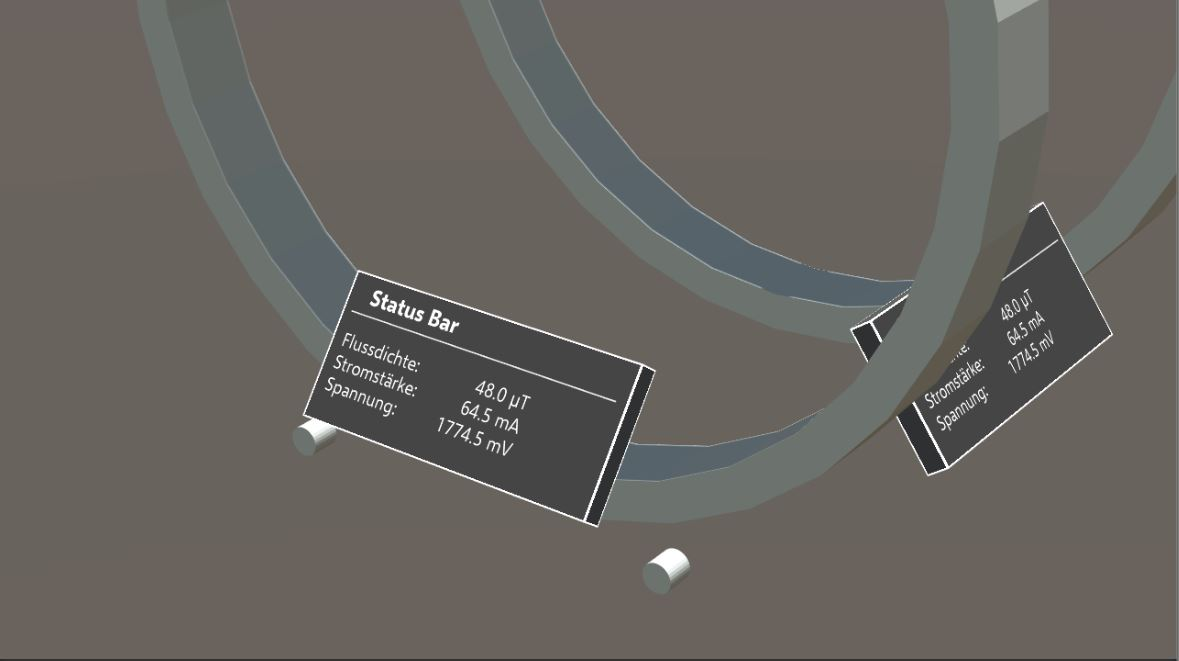
\includegraphics[width=0.4\textwidth]{images/unity/status.jpg}
	\caption{Darstellung der numerischen Werte.}
	\label{img:status}
\end{wrapfigure}

Die Positionierung an den Verbindungsstücken liegt, wie auch bei den Indikatoren für die Stromrichtung, im Ausnutzen von Platz begründet. Die Objekte sind schräg gestellt (ca. 35°), so dass sie aus diesem typischen Winkel gut zu lesen sind.\\

Durch ihre Platzierung unmittelbar über dem Untergrund würden Drop Shadows das Präsenzgefühl stärken. Diese lassen sich hier jedoch nicht direkt umsetzen, denn der Untergrund ist real und kann durch die HoloLens nicht weiter verdunkelt werden. Eine mögliche Lösung bestünde darin, die Schatten zu erzeugen, indem der Untergrund außerhalb des Schattens zusätzlich erhellt wird. Allerdings müssten hier wiederum die Schatten der realen Objekte mit einbezogen werden. Daher nimmt diese Lösung die fehlenden Schatten in Kauf.\\

Man könnte auch eine Lösung über UI-Elemente in Erwägung ziehen, da es sich um numerische Werte ohne einen natürlichen Ankerpunkt in der Szene handelt. Allerdings sind solche Lösungen aus verschiedenen Gründen auf der HoloLens ungünstig. Fest im Bild positionierte Elemente wären aufgrund der Vibrationen des Kopfes kaum bis gar nicht lesbar. Eine Stabilisierung auch über Kopfbewegungen hinweg nimmt wiederum Platz in Anspruch. Außerdem würde eine solche Realisierungen zusätzliche Fokuswechsel nach sich ziehen. Deshalb rät die Dokumentation explizit vom Gebrauch solcher Elemente ab und hier die Variante eines fest stehenden Objektes gewählt.\\

\vspace{8px}
\begin{center}
	\fbox{
		\parbox{0.9\linewidth}{
			\vspace{4px}
			\textbf{Zusammenfassung}
			\begin{itemize}[rightmargin=12px, topsep=-12px]
				\setlength{\itemsep}{-1pt}
				\singlespacing
				\item Stromstärke (gemessen) und Flussdichte (berechnet) werden auf einem Datenpanel dargestellt
				\item Platzierung an unteren Balken zwischen den Spulen nutzt das Sichtfeld aus
				\item Sichtbarkeit analog zu Strom-Pfeilen
				\item Dunkelgrauer Hintergrund für bessere Lesbarkeit
			\end{itemize}
			\vspace{18px}
	}}\\
\end{center}
\vspace{6px}

\subsubsection{Zusammenfassung}
Nachdem in den vorangegangenen Abschnitten die einzelnen Elemente vorgestellt wurden soll das visuelle Design anhand von Fotos von der HoloLens zusammengefasst werden. Bei der Bewertung der Abbildungen ist jedoch die eingeschränkte Qualität zu beachten. Die tatsächliche Darstellungsqualität auf der HoloLens entspricht den zuvor gezeigten Screenshots aus der Entwicklungsumgebung. Einen ersten Eindruck der zusammengesetzten Darstellungen auf der HoloLens gibt Abbildung \ref{img:hl_ss_intro}.\\

\begin{figure}[h!]
	\centering
	\includegraphics[width=0.39\textwidth]{images/HL/fieldlines.jpg}
	\hspace{0.01\textwidth}
	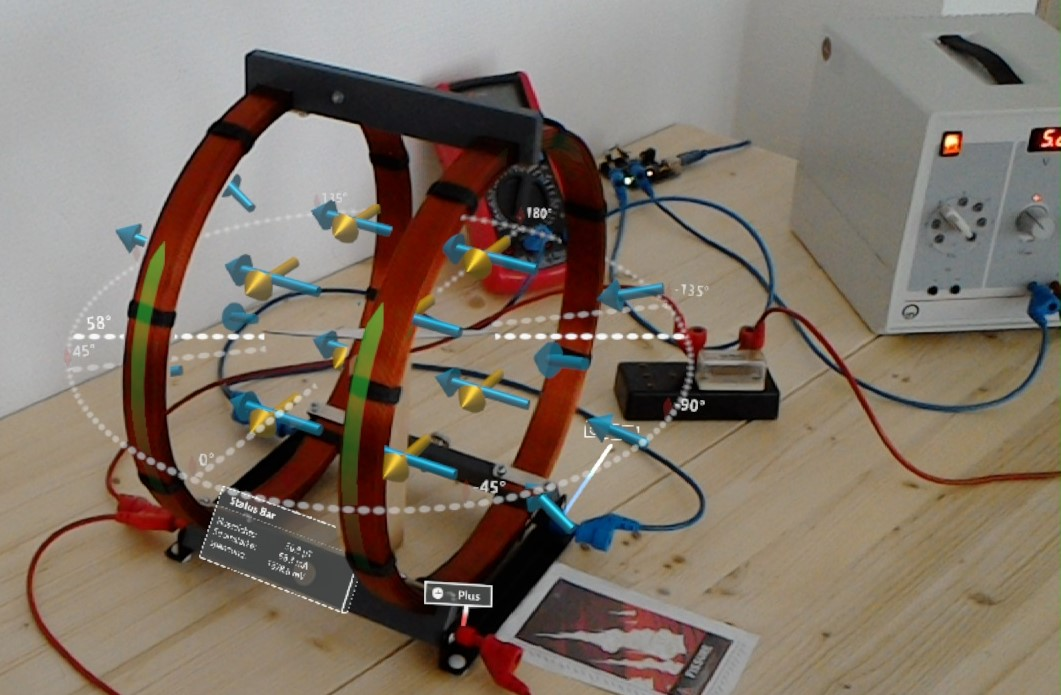
\includegraphics[width=0.55\textwidth]{images/HL/Vektoren.jpg}
	\caption{Aufnahmen der beiden Echtzeitdarstellungen von der HoloLens }
	\label{img:hl_ss_intro}
\end{figure}

TODO...\\

\begin{figure}[h!]
	\centering
	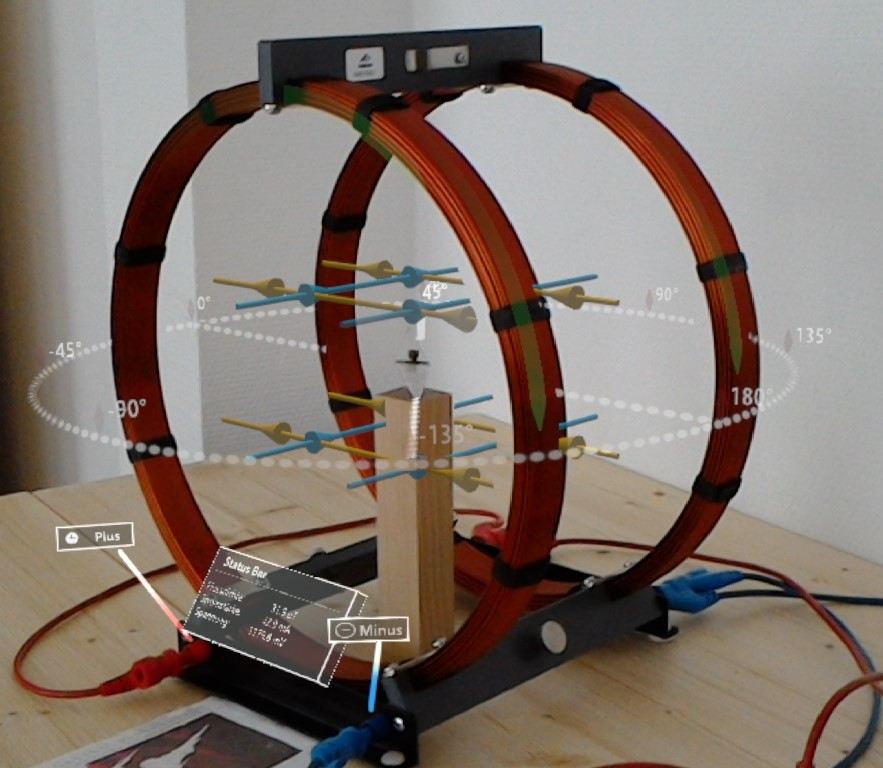
\includegraphics[width=0.37\textwidth]{images/HL/45DegCut.jpg}
	\hspace{0.01\textwidth}
	\includegraphics[width=0.57\textwidth]{images/HL/compass.jpg}
	
	\vspace{0.01\textwidth}
	
	\includegraphics[width=0.48\textwidth]{images/HL/simulation.jpg}
	\hspace{0.01\textwidth}
	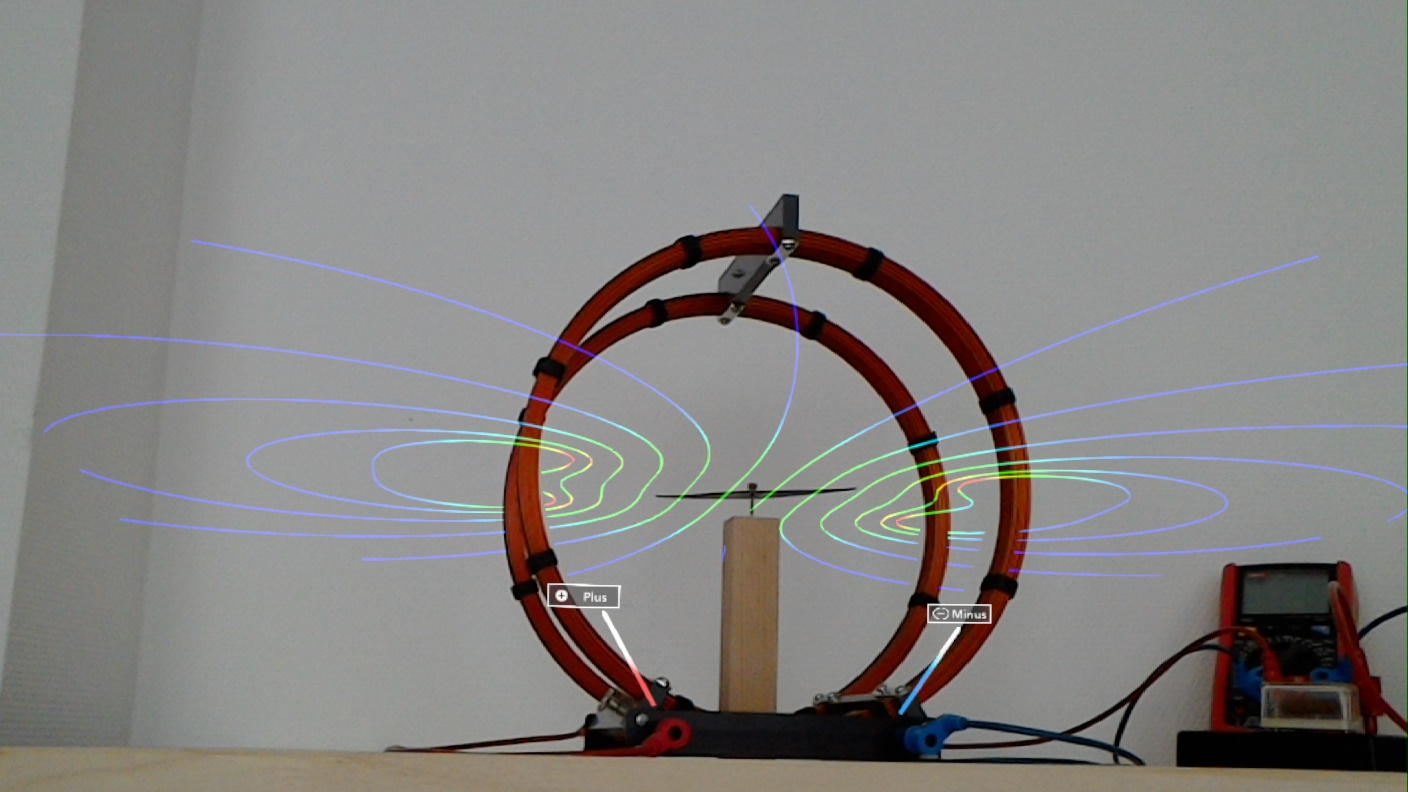
\includegraphics[width=0.48\textwidth]{images/HL/simu2.jpg}
	\caption{Oben: Auslenkung der Magnetnadel im Vergleich zur 45° Linie und zur theoretischen Auslenkung. Unten: Simulationsdarstellung.}
	\label{img:hl_ss}
\end{figure}


\subsection{Interaktion}
\label{sec-4-4}
Die Interaktion soll möglichst einfach gehalten werden und auch für Nutzer ohne Erfahrung mit der HoloLens geeignet sein. Daher folgt das Design der Empfehlung, alternative Interaktionsmöglichkeiten zur Verfügung zu stellen. Diese Lösung bietet dem Anwender drei Eingabemethoden an:
\begin{enumerate}
	\setlength{\itemsep}{-5pt}
	\item Klicker
	\item Handgesten
	\item Sprachbefehle
\end{enumerate}

Der Klicker ist ein kleiner, in der Hand gehaltener Taster, der sich wie eine Maustaste verhält. Ein mal drücken wird als Klick erkannt, aber auch gedrückt halten ist möglich.
Die dazu korrespondierende Handgeste ist der AirTap, der auf der HoloLens als Klick-Geste dient. Als Klick erkennt das Gerät außerdem den reservierten Sprachbefehl ''Select''. Weitere Sprachbefehle werden von der Anwendung selbst definiert.\\

Die Lösung stellt dem Anwender die drei Eingabemethoden frei zur Verfügung. Das bedeutet, der Nutzer kann selbst entscheiden, auf welche Methoden er zurückgreift. Jede Interaktionsmöglichkeit kann jederzeit genutzt werden. Anwender, die keine Erfahrung mit der HoloLens haben, sind nicht gezwungen, zunächst die Gestensteuerung der HoloLens zu erlernen. Außerdem ist die Interaktion so auf natürliche Weise konsistent: Ein Klick mit dem Klicker ist äquivalent zu einem Klick durch die AirTap-Geste.\\

Während der Durchführung des Versuches sind drei Aktionen möglich:
\begin{enumerate}[topsep=-2px]
	\setlength{\itemsep}{-5pt}
	\item Veränderung des Stromflusses über den Regler der Spannungsquelle
	\item Wechsel zwischen den Darstellungsmodellen
	\item Rückkehr zum Hauptmenü
\end{enumerate}
\vspace{8px}

Bei ersterer interagiert der Nutzer mit dem Versuchsaufbau, die Anwendung passt sich dabei automatisch an den sich ändernden Stromfluss anhand der Messwerte an. Für den Wechsel zwischen den Darstellungen sowie die Rückkehr zum Menü werden die zuvor beschriebenen Möglichkeiten angeboten. In jedem Fall reagiert die Anwendung mit visuellem oder akustischem Feedback auf ein Kommando.\\

\begin{comment}
\textbf{Menü, Einstellungen und Tracking}\\
Das Menü und die Einstellungen werden über Buttons gesteuert. Diese lassen sich über den standardmäßigen Cursor in der Mitte des Sichtfeldes anvisieren und dann mit einem Klick betätigen. Der Cursor ist jedoch nur während der Nutzung des Menüs oder der Einstellungen sichtbar, da sonst keine Objekte ausgewählt werden müssen und der Cursor zwischen den anderen Hologrammen nur stören würde. Länger laufende Operationen wie z.B. das Laden von Objekten werden außerdem durch einen Progress Indikator mit einem kurzen Text angezeigt.\\

Die Lösung baut hier auf den vorhandenen Elementen des MRTK auf und nutzt vorgefertigte Objekte. Dazu gehören Cursor, Progress Indikator, das virtuelle Keyboard und Buttons. Dadurch entsteht zum einen eine konsistente Interaktionsweise. Zum anderen sind die Komponenten speziell für die HoloLens designet und bringen bereits gewünschtes Verhalten wie z.B. Feedback bei Aktionen bereits mit.
\\
\vspace{8px}
\begin{center}
	\fbox{
		\parbox{0.9\linewidth}{
			\vspace{4px}
			\textbf{Überblick}
			\begin{itemize}[rightmargin=12px, topsep=-12px]
				\setlength{\itemsep}{-1pt}
				\singlespacing
				\item Interaktion mittels Klicker, Handgesten und Sprache
				\item Jede Methode kann jederzeit genutzt werden
				\item Visuelles oder akustisches Feedback für Nutzereingaben
				\item Verwendung vorgefertigter, für die HoloLens designeter Objekte
			\end{itemize}
			\vspace{18px}
	}}\\
\end{center}
\vspace{6px}
\end{comment}

\subsection{Designentscheidungen im Hinblick auf die Implementierung}
\label{sec-4-3}
Die Lösung sieht neben den inhaltlichen Darstellungen weitere Komponenten vor, die der Nutzbarkeit der Anwendung dienen. Das betrifft drei Bereiche: Die Steuerung des Ablaufes, die Bestimmung von Position und Ausrichtung der Spule sowie Einstellungen.\\

\textit{Menü}\\
Über ein Menü kann der Ablauf der Anwendung gesteuert werden. Hier kann der eigentliche Versuch gestartet, die Positionsbestimmung (erneut) angestoßen oder die Einstellungen aufgerufen werden. Die Umsetzung erfolgt über Buttons, die sich automatisch der Kamera anpassen, so dass der Anwender keine Probleme hat, sie zu finden.\\

\textit{Einstellungen}\\
Die Einstellungen bieten die Konfiguration wichtiger Parameter an. Das betrifft vor allem die gemessene Flussdichte des Erdmagnetfeldes, da sich diese von Ort zu Ort unterscheiden kann. Aber auch der gewählte Widerstand lässt sich einstellen, da hier ein Austausch in der Schaltung leicht möglich und beim Wechsel auf eine andere Spannungsquelle unter Umständen sogar nötig ist. Auch die Einstellung der Adresse des Servers, von dem die Messwerte abgefragt werden, wird angeboten. Die Eingabe der Werte erfolgt dabei über die vom Mixed Reality Toolkit zur Verfügung gestellte, virtuelle Tastatur.\\

Damit die Einstellungen nicht nach jedem Neustart der Anwendung vorgenommen werden müssen, sieht die Lösung eine Speicherung auf dem lokalen Speicher der HoloLens vor. Bei der erstmaligen Verwendung werden Default-Werte geladen, auf die die Applikation auch wieder zurückgesetzt werden kann. Die Einstellungen tragen somit wesentlich zur Nutzbarkeit der Anwendung bei. Ohne diese Optionen müsste die App für jede Änderung in diesen Parametern mit der geänderten Konfiguration neu deployt werden. Insbesondere bei der Adresse des Servers wäre dies problematisch, da diese, je nach technischer Umsetzung, ggf. zum Zeitpunkt des Deployments noch gar nicht bekannt ist.\\

\textit{Tracking}\\
Nicht zuletzt soll die Anwendung den Nutzer durch den Prozess der Positionsbestimmung der Spule führen. Die Bestimmung erfolgt über einen optischen Marker, der über die integrierte Kamera eingelesen wird. Die Verwendung eines hinreichend großen Markers erlaubt die Genauigkeit im Bereich weniger Millimeter, die von der Anwendung benötigt wird. Letztere instruiert den Nutzer dabei und informiert über den Fortschritt des Vorgangs.\\
\noindent\hspace*{5mm}
Die Idee dahinter besteht darin, diesen, hier als ''Tracking'' bezeichneten Vorgang, nur einmalig erfolgen zu lassen. Wurden Position und Ausrichtung einmal ermittelt, werden diese gespeichert und verwendet. Hier bietet die HoloLens den sogenannten \textit{World Anchor Store} an, in dem die Position von Objekten in Relation zum Raumverständnis dauerhaft gespeichert werden kann. Dieser Speicher ist persistent und kann die Position über mehrere Anwendungssessions hinweg speichern.\\
 
Das Design nutzt hier gezielt die Funktionalitäten der HoloLens sowie den Umstand aus, dass Spule und Magnetnadel, nachdem sie einmal aufgestellt wurden, nicht weiter bewegt werden müssen. Allerdings bedeutet dieser Ansatz auch, dass die Qualität der Positionierung über mehrere Sessions hinweg abhängig vom Raumverständnis der HoloLens ist. Deshalb lässt sich das Tracking jederzeit manuell neu anstoßen, wenn die Überlagerung als nicht gut genug empfunden wird.\\

Solange also der Versuchsaufbau nicht bewegt wird, kann die einmalig gespeicherte Position verwendet werden. Die Anwendung erkennt automatisch, ob die gespeicherten Daten vorliegen. Dadurch verkürzt sich die Setup-Zeit und es trägt dazu bei, dass auch unerfahrene Nutzer die Applikation verwenden können.

\vspace{8px}
\begin{center}
	\fbox{
		\parbox{0.9\linewidth}{
			\vspace{4px}
			\textbf{Zusammenfassung}
			\begin{itemize}[rightmargin=12px, topsep=-12px]
				\setlength{\itemsep}{-1pt}
				\singlespacing
				\item Start-Logo mit Ladevorgang
				\item Menü mit Start der Hauptanwendung, Tracking und Optionen, jederzeit aufrufbar
				\item Einstellungsmenü für IP, Feldstärke der Erde und weitere Parametern, Default-Werte vorhanden
				\item Einstellungen werden persistent auf der HoloLens gespeichert und lassen sich ggf. auf Default-Werte zurücksetzen
				\item Tracking-Sequenz zum Einlesen des Markers mit persistenter Speicherung der Position
			\end{itemize}
			\vspace{18px}
	}}\\
\end{center}
\vspace{6px}

Das folgende Kapitel erläutert nun die Details der Umsetzung dieser Lösung.

